\subsection{Abgleich des Tastkopfes}\label{sec:2-4}

\begin{highlightblock}[Abgleich des Tastkopfes bei DC-Kopplung]
	\begin{enumerate}[label=\textbf{\alph*:}, ref=\alph*]
		\item\label{itm:2-P4-1} Abgleich des Tastkopfes (Rechtecksignal)
		\item\label{itm:2-P4-2}Ersatzschaltung (10:1-Tastkopf, DC-Kopplung) (Abb.~\ref{fig:impedanz-oszi-taskopf}) \\
		      Tastkopf $R_T = \SI{9}{\mega\ohm} \,||\, C_T$, in Serie zum Oszilloskopeingang ($\SI{1}{\mega\ohm} \,||\, \SI{20}{\pico\farad}$). Mit Kabelkapazität $C_K = \SI{100}{\pico\farad}$
		\item\label{itm:2-P4-3} Berechnung der Eingangsimpedanz bei 1 MHz
	\end{enumerate}

\end{highlightblock}

\subsubsection{Verwendetes Material}

\begin{table}[h]
	\centering
	\caption{Verwendetes Material}
	\begin{tabularx}{\textwidth}{XXX}
		\textbf{Messgerät} & \textbf{Verwendung} & \textbf{Anmerkungen}                                \\ \midrule
		TDS2014C           & Oszilloskop         & $Z_E = \SI{1}{\mega\ohm}\,||\,\SI{20}{\pico\farad}$ \\
	\end{tabularx}
\end{table}

\marginref{\ref{itm:2-P4-1}} Abgleichen des Tastkopfes

Hier wird die Kapazität im Tastkopf so verstellt, dass bei $U_E$=Rechtecksignal das Oszilloskop ein schönen unverzerrtes Rechtecksignals wie in Abb.~\ref{fig:oszi-tastkopf-testsignal} anzeigt. Überschwingt das Signal, so ist $C_T$ zu klein, ist das Rechteck an den vorderen Flangekn abgerundet, so ist $C_T$ zu groß.

\marginref{\ref{itm:2-P4-2}} Die Ersatzschaltung ist in Abb.~\ref{fig:impedanz-oszi-taskopf} zu sehen.

\begin{figure}[h]
	\begin{minipage}[t]{.45\textwidth}
		\centering
		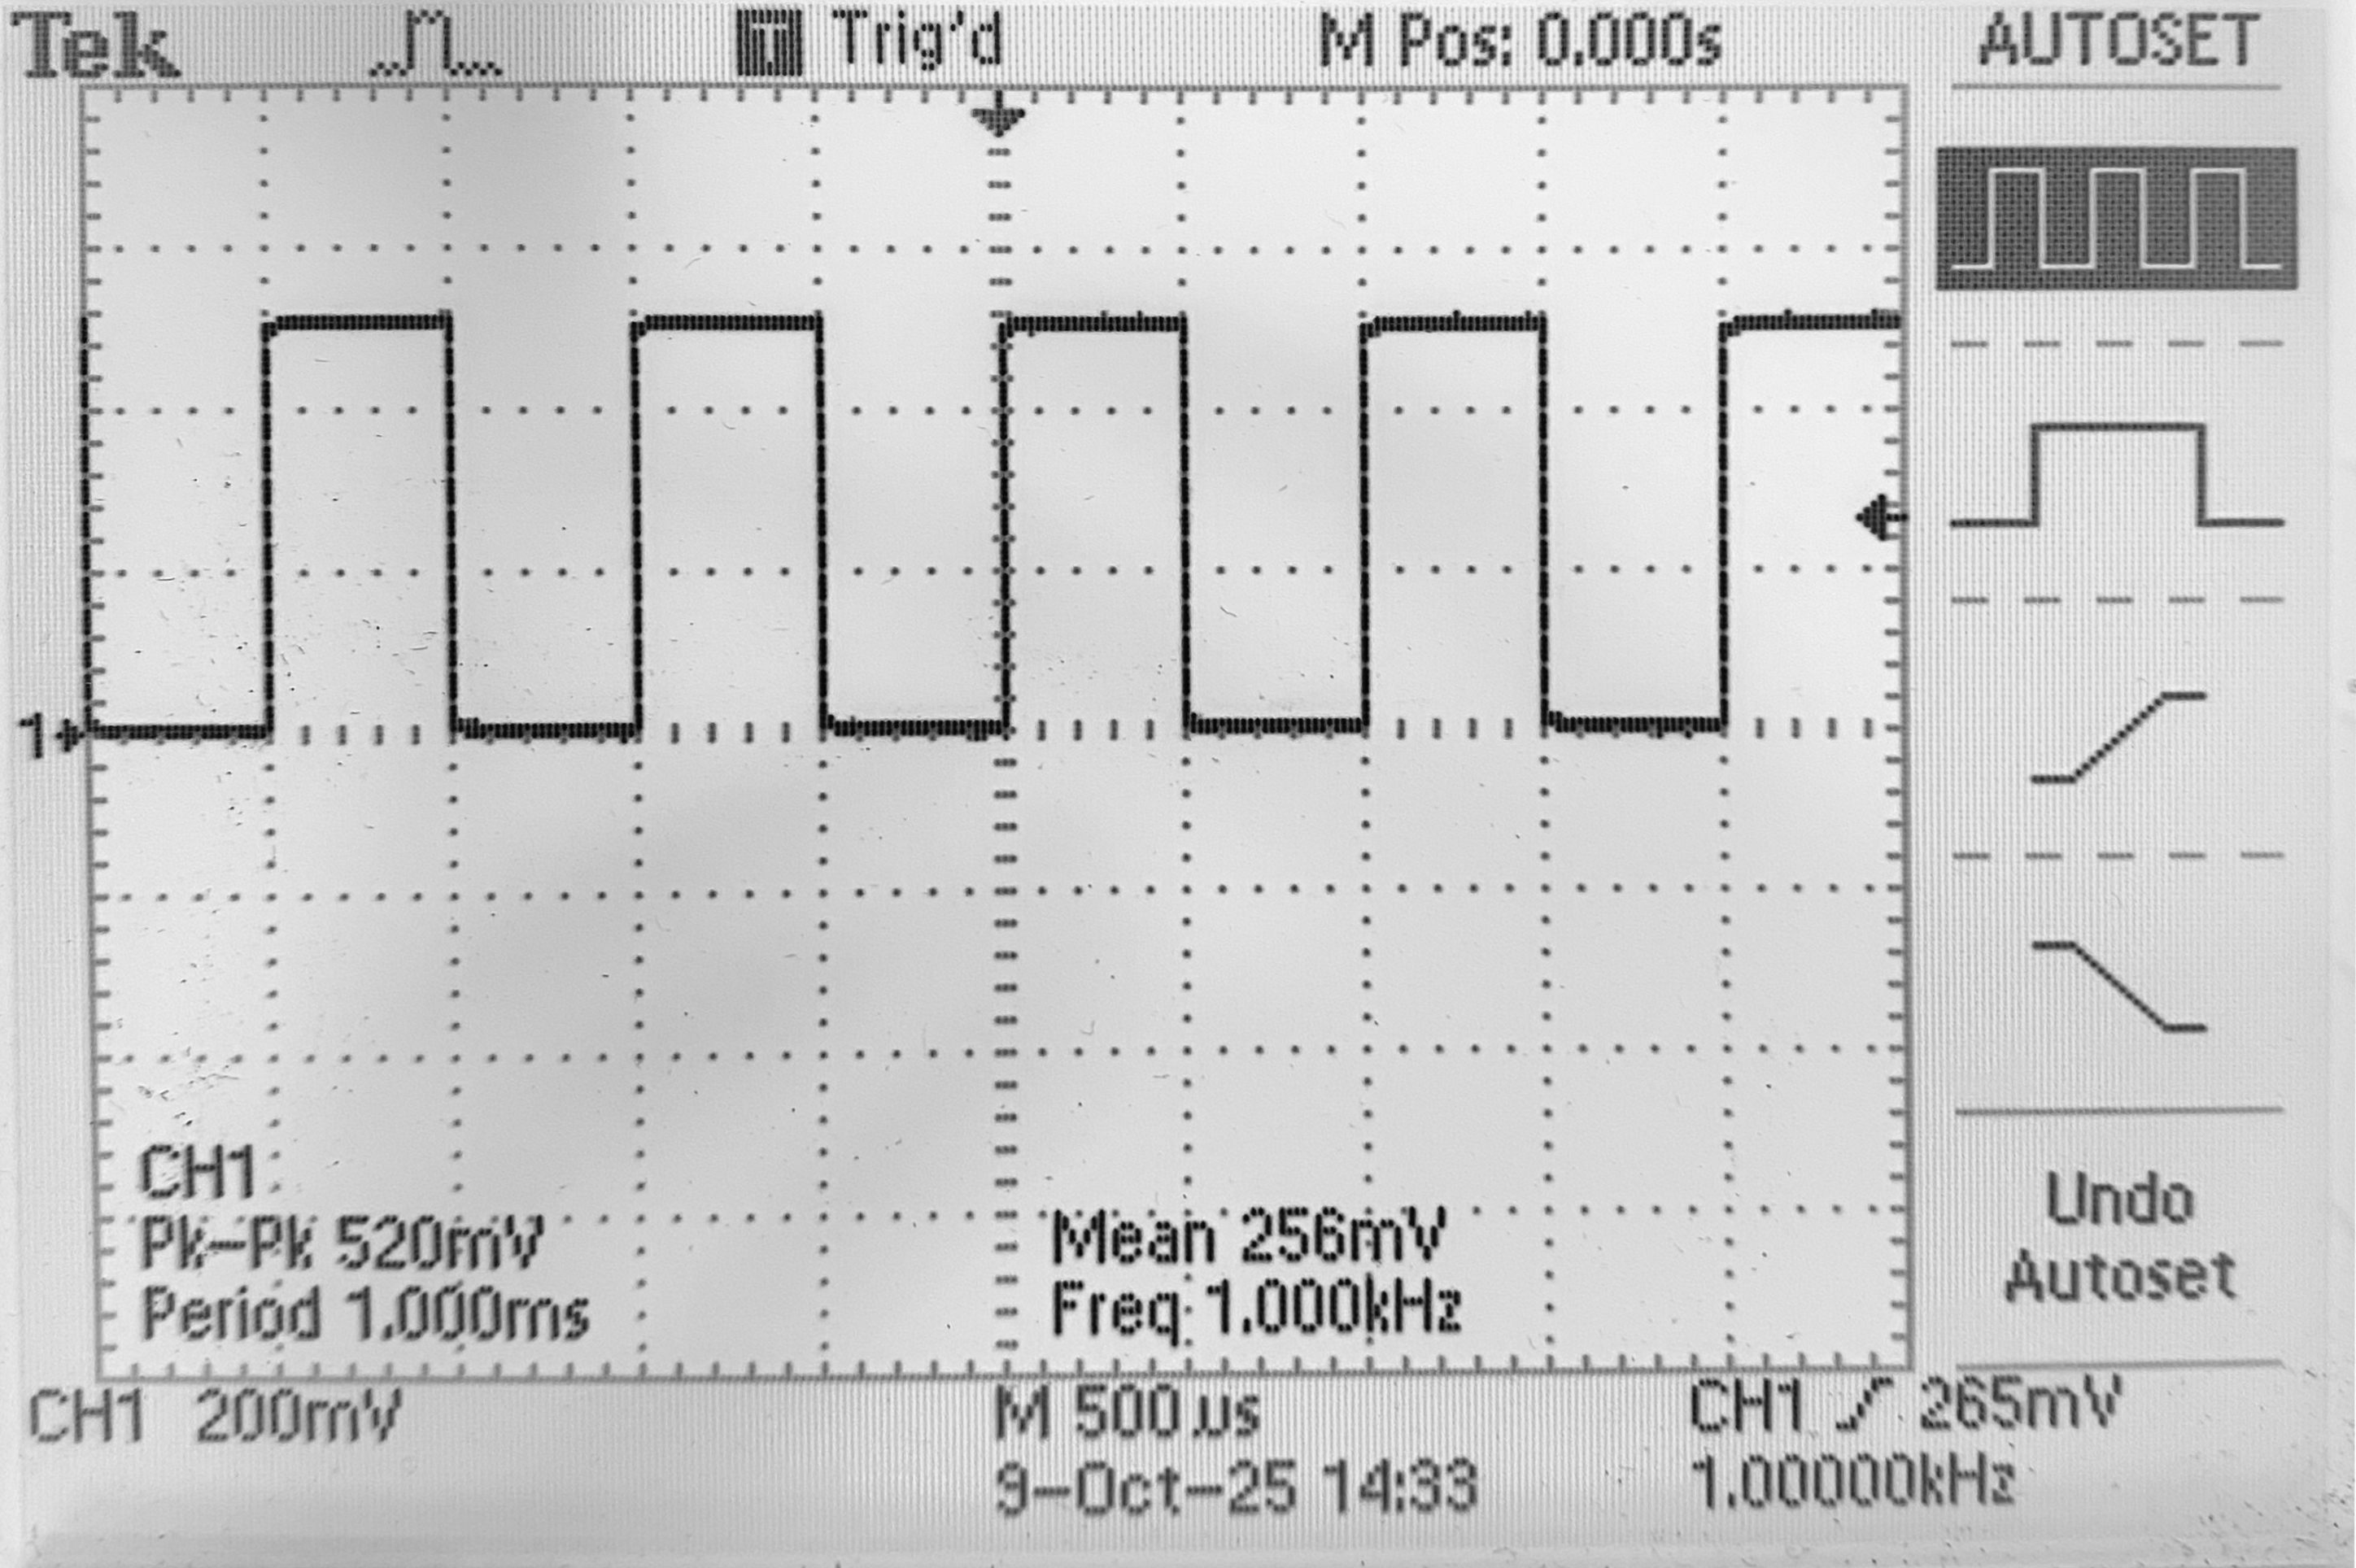
\includegraphics[height=4.8cm]{images/TastkopCal.JPEG}
		\caption{Abgleich eines Tastkopfes am Oszilloskop mittels Testsignal}\label{fig:oszi-tastkopf-testsignal}
	\end{minipage}\hfill
	\begin{minipage}[t]{.48\textwidth}
		\centering
		\begin{circuitikz}[scale=0.75, transform shape]
			% Eingangsspannung
			\draw (0,0) node[ocirc]{}
			(0,4) node[ocirc]{};
			\draw[<-] (0,0.3) -- (0,3.7) node[midway,left]{$U_E$};

			% Bauteile
			\draw (1,5) to[R, l=$R_{T}$] (3,5) coordinate (k1);
			\draw (1,3) to[variable capacitor, l=$C_{T}$] (3,3) coordinate (k2);
			\draw (5,0) to[C, l=$C_K$]   (5,4) coordinate (k3);
			\draw (7,0) to[C, l=$C_E$]   (7,4) coordinate (k4);
			\draw (9,0) to[R, l=$R_E$]   (9,4) coordinate (k5);

			% Kabel horizontal
			\draw (0,0) -- (9,0);
			\draw (0,4) -- (1,4);
			\draw (3,4) -- (9,4);
			% Kabel vertical
			\draw (1,3) -- (1,5);
			\draw (3,3) -- (3,5);
		\end{circuitikz}
		\captionof{figure}{Eingangsimpedanz des Oszilloskops bei AC-Kopplung}\label{fig:impedanz-oszi-taskopf}
	\end{minipage}
\end{figure}



\marginref{\ref{itm:2-P4-3}} Berechnung der Eingangsimpedanz bei 1 MHz

Aus der Abgleichbedinung $R_T C_T = R_E \tilde{C_E}$ kann man sich $C_T$ berechnen mit $\tilde{C_E} = C_E + C_K$.

\begin{align}
	 & C_T        = \frac{R_E}{R_T}(C_E + C_K) = \frac{\SI{1}{\mega\ohm}}{\SI{9}{\mega\ohm}}(\SI{20}{\pico\farad} + \SI{100}{\pico\farad}) = \SI{13.3}{\pico\farad} \\
	 & Z_{ges}    = Z_T + \tilde{Z_E} = \frac{R_T}{1+j\omega R_T C_T} + \frac{R_E}{1+j\omega R_E (C_k+C_E)} = \SI{17.67}{\ohm} - j\SI{13292.81}{\ohm}               \\
	 & |Z_{ges}|  = \SI{13292.82}{\ohm} \label{eq:eingangswiderstand_oszi_mit_taskopf}
\end{align}

\subsubsection{Erkenntnisse}
Mit dem Tastkopfe (Gl.~\ref{eq:eingangswiderstand_oszi_mit_taskopf}) ist $|Z_{ges}|$ ca. 10-mal so groß wie ohne (Gl.~\ref{eq:eingangswiderstand_oszi}). Dadurch ver-10-facht sich auch der Messbereich des Oszilloskops, was für große Signale notwendig ist. Allerdings verringert es auch die Empfindlichkeit was die Messung kleiner Signale ungenauer macht.

